\section{Auswertung}


\subsection{Vermessung der Nanostruktur}



\begin{figure}
  \centering
  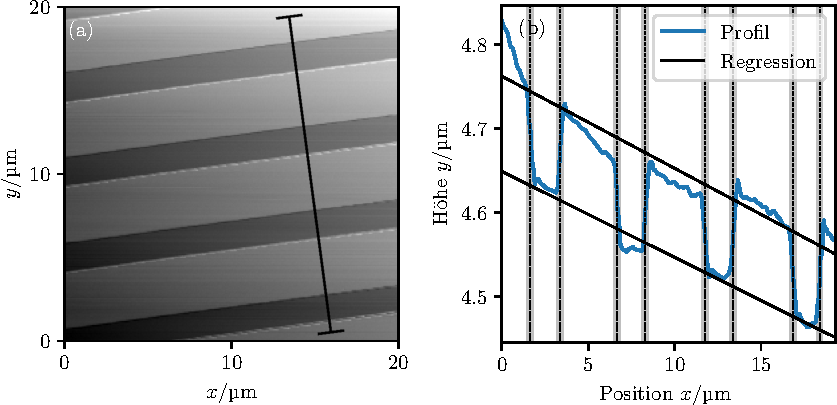
\includegraphics[scale = 1]{../analysis/data/nanostruktur_linien/linien_profil.pdf}
  \caption{Ergebnis der Messung an dem Linienprofil der Nanostruktur. (a) AFM Aufnahme mit eingezeichneten
  Linien, enlang derer das Profil in Abbildung (b) aufgenommen wurden. Das Profil ist
  über die Breite der in (a) eigezeichneten Balken gemittelt. Zudem sind in (b) die linearen Regressionen
  an die Datenpunkte eingezeichnet, die dem oberen bzw. unterem Niveau der Nanostruktur zugeordnet wurden.}
  \label{fig: linien_profil}
\end{figure}



\begin{figure}
  \centering
  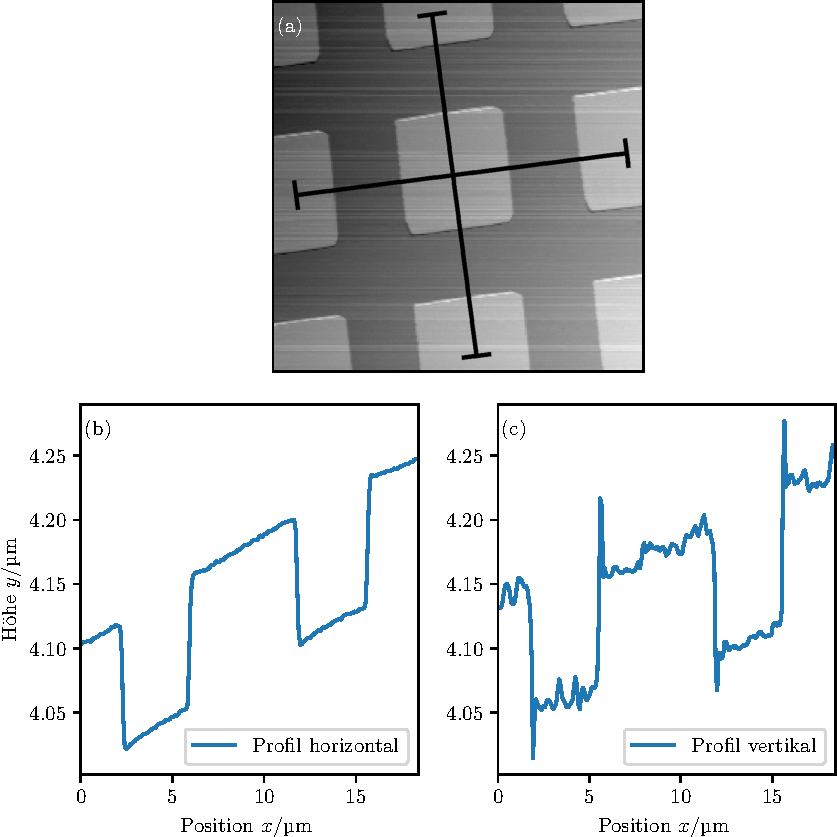
\includegraphics[scale = 1]{../analysis/data/nanostruktur_quadrate/quadrate_profile.pdf}
  \caption{Ergebnis der Messung an den quadratischen Nanostrukturen. (a) AFM Aufnahme mit eingezeichneten
  Linien, enlang derer die Profile in Abbildung (b) und (c) aufgenommen wurden. Die Profile sind
  über die Breite der in (a) eigezeichneten Balken gemittelt.}
  \label{fig: quadrate_profil}
\end{figure}



\begin{figure}
  \centering
  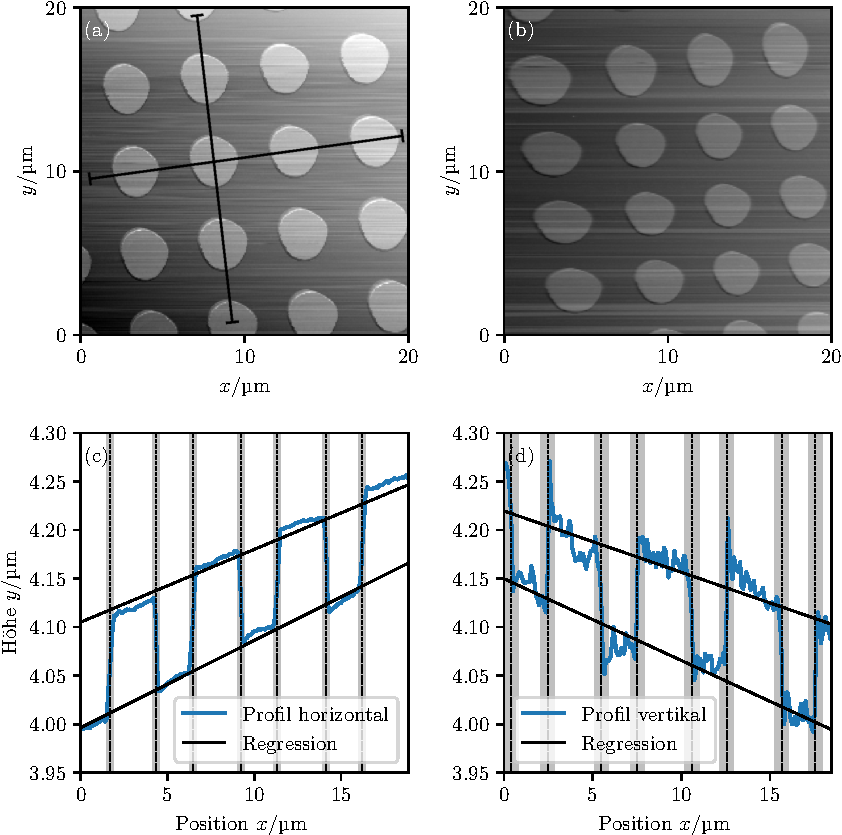
\includegraphics[scale = 1]{../analysis/data/nanostruktur_kreise/kreise_profile.pdf}
  \caption{}
  \label{fig: kreise_profil}
\end{figure}

\subsection{Kraft-Abstands-Kurven}
Abbildung~\ref{fig: force_distance} zeigt zum qualitativen Vergleich der auftretenden Kraft Werte die drei aufgenommenen Kraft-Abstands-Kurven der Proben
Edelstahl, DLC und Teflon. Zur Diskussion des generellen Verlaufs einer solchen Kurve, ist in Abbildung~\ref{fig: force_distance_teflon} die Kurve
für Teflon vergrößert dargestellt und die verschiedenen Bereiche beschriftet.

Zur Bestimmung des Elastizitätsmoduls von Teflon werden die Bereiche rechts von dem Snap-in betrachtet. Diese Daten aus den drei Kurven sind
in Abbildung~\ref{fig: depth} noch einmal aufgetragen, wobei der Ursprung jeweils in den Snap-in Punkt gelegt wurde. Die Daten sind
jeweils nur bis zu einem gemeinsamen maximalen Verschiebungspunkt gezeichnet.
Die beiden Kurven von Edelstahl und DLC überlagern sich gänzlich (siehe (c)), da beide Materialien undeformierbar sind.
Es ist deutlich zu erkennen, dass
die Steigung der Geraden von Teflon geringer ist als die von DLC und Edelstahl, was auf das Eindringen der Spitze in die Probe zurückzuführen ist.
Die Eindringtiefe am maximalen Verschiebungspunkt kann gewonnen werden, indem der horizontale Abstand der beiden Kurven in den Abbildungen~\ref{fig: depth}
(a) und (b) gemessen wird. Die Eindringtiefe $\delta$ entspricht dem Abstand der beiden eingezeichneten vertikalen Linien.
Es ergeben sich die Werte
\begin{equation}
  \text{(a): } \delta \approx \SI{0.13}{\micro\meter} \quad \text{und (b): }\delta \approx \SI{0.070}{\micro\meter}.
\end{equation}
Gemäß Formel~\eqref{} kann daraus das Elastizitätsmodul $E$ gewonnen werden.
\begin{equation}
  \text{(a): } E \approx \SI{120}{\mega \pascal} \quad \text{und (b): } E \approx \SI{260}{\mega \pascal}.
\end{equation}
In Quelle~\cite{} ist der Wert
\begin{equation}
  E\ua{lit} = \SI{420}{\mega \pascal}
\end{equation}
zu finden.

Abschließend kann die maximal wirkende Adhäsionskraft bestimmt werden. Hierzu wird der horzontale
Abstand zwischen dem Pull-off und Snap-in mit der Federkonstante des Cantilevers multipliziert.
Für die drei Proben ergeben sich die folgenden Werte:
\begin{align}
  \begin{aligned}
    \text{Edelstahl: } & F\ua{adh} &\approx \\
    \text{DLC: } & F\ua{adh}       &\approx \\
    \text{Teflon: } & F\ua{adh}    &\approx
  \end{aligned}
\end{align}



    \the\textwidth
    \the\textheight
\begin{figure}
  \centering
  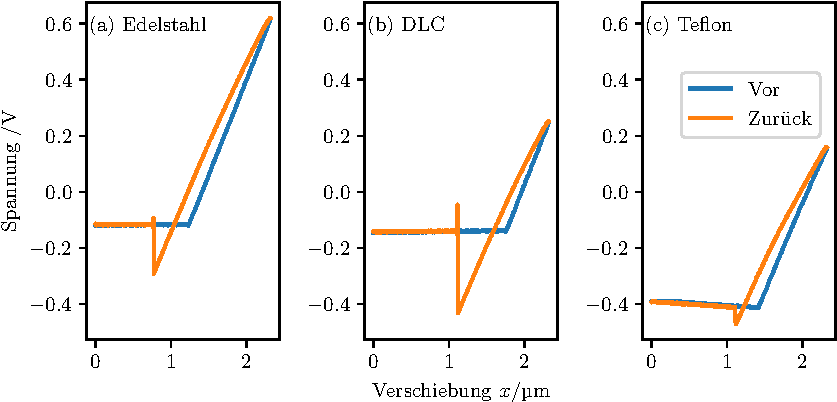
\includegraphics[scale = 1]{../analysis/data/force_distance/force_distance.pdf}
  \caption{Vergleich der drei aufgenommenen Kraft-Distanz-Kurven.}
  \label{fig: force_distance}
\end{figure}
